\documentclass{article}
\usepackage{tikz}
\usetikzlibrary{positioning}

\begin{document}

\begin{center}
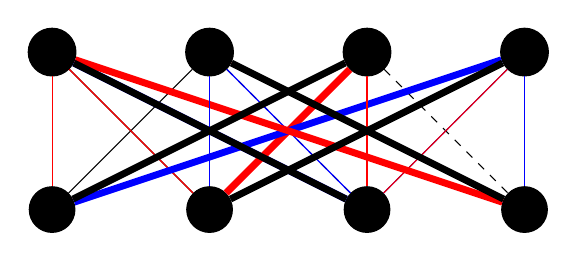
\begin{tikzpicture}[scale=0.5]
  \tikzset{
    vertex/.style = {circle,fill,draw,inner sep=2pt},
  }
  
  % Define vertices
  \node[vertex] (u1) at (-4,0) {$u_1$};
  \node[vertex] (u2) at (0,0) {$u_2$};
  \node[vertex] (u3) at (4,0) {$u_3$};
  \node[vertex] (u4) at (8,0) {$u_4$};
  
  \node[vertex] (v1) at (-4,-4) {$v_1$};
  \node[vertex] (v2) at (0,-4) {$v_2$};
  \node[vertex] (v3) at (4,-4) {$v_3$};
  \node[vertex] (v4) at (8,-4) {$v_4$};
  
  
  % Draw edges
  \draw (u1) -- (v2);
  \draw (u2) -- (v1);
  \draw[dashed] (u2) -- (v3);
  \draw[dashed] (u3) -- (v4);
  
  \draw[dashed] (u1) -- (v3);
  \draw[dashed] (u3) -- (v2);
  \draw[dashed] (u4) -- (v3);
  \draw[dashed] (u4) -- (v4);
  

  \draw[red] (u2) -- (v2);
  \draw[red] (u3) -- (v1);
  \draw[blue] (u1) -- (v4);
  \draw[blue] (u4) -- (v3);
  
  % Drawing the second round
  \begin{scope}[xshift=10cm]
    
    \draw[red] (u1) -- (v2);
    \draw[blue] (u2) -- (v3);
    \draw[red] (u2) -- (v4);
    \draw[blue] (u3) -- (v1);
    \draw[blue] (u3) -- (v2);
    \draw[red] (u4) -- (v3);
    \draw[red] (u4) -- (v4);
    
    \draw[blue, line width=2.5pt] (u1) -- (v3);
    \draw[red, line width=2.5pt] (u3) -- (v2);
    \draw[blue, line width=2.5pt] (u4) -- (v1);
    \draw[red, line width=2.5pt] (u1) -- (v4);
  \end{scope}
  
  
  % Drawing the third round
  \begin{scope}[xshift=20cm]
    \draw[red] (u1) -- (v1);
    \draw[blue] (u2) -- (v2);
    \draw[red] (u3) -- (v3);
    \draw[blue] (u4) -- (v4);
    
    \draw[line width=2.5pt] (u2) -- (v4);
    \draw[line width=2.5pt] (u3) -- (v1);
    \draw[line width=2.5pt] (u4) -- (v2);
    \draw[line width=2.5pt] (u1) -- (v3);
  \end{scope}
\end{tikzpicture}
\end{center}

In order to build a perfect matching in \( K_{4,4}^- \), in each round the Waiter offers the two dashed edges.